% 2017 KTS
% 텍 매크로 작성법

\documentclass{beamer}

\usetheme{metropolis}
\metroset{outer/progressbar=head}

\usepackage{fancyvrb}
\usepackage{kotex}
\hypersetup{pdfencoding=auto}


% title
\title{\TeX\ 매크로}
\subtitle{매크로 작성의 기초와 예제}
\date{2017년 2월 11일 토요일}
\author{남수진}
\institute{
  2017 한국텍학회 학술대회 및 정기총회 \\
  동국대학교 법학관 B253호}
\titlegraphic{\hfill
\includegraphics[height=3cm]{meta.pdf}}


%%
\begin{document}

\maketitle

%
\begin{frame}[standout]
  Plain \TeX
\end{frame}

%
\begin{frame}[fragile]{매크로 정의}
  \medskip
  \hbox to\hsize{\hss
    \verb+\def+<control sequence>\alert{<parameter text>}%
    \verb+{+\alert{<replacement text>}\verb+}+\hss}
  \smallskip
  \begin{itemize}
  \item 문서에서 여러 번 반복되어 사용되는 문구나 일련의 명령어의 나열을
    하나의 명령어(control sequence)로 만든 것
  \item \verb+\def+, \verb+\gdef+, \verb+\edef+, \verb+\xdef+
  \item 라텍의 \verb+\newcommand+, \verb+\newenvironment+
    \begin{Verbatim*}[fontsize=\small, formatcom=\color{blue}]
\def\xvec{(x_1,\ldots,x_n)}
\def\row#1{(#1_1,\ldots,#1_n)}
\def\cs #1. #2\par{...}
\cs You owe \$5.00. Pay it.\par
    \end{Verbatim*}
  \item 텍의 처리 과정 중에서, \alert{전개 과정}에서 매크로는 치환 텍스트로 전개된다.
  \end{itemize}
\end{frame}


%
\begin{frame}{텍의 처리 과정}  
  \begin{itemize}
  \item \alert{\bf 입력(Input)} 파일을 줄(line) 단위로 읽어서
    \alert{토큰 리스트}를 만든다.
  \item \alert{\bf 전개(Expansion)} 위의 토큰 리스트를 입력으로
    받어서 전개할 수 있는
    모든 토큰을 전개해서 더이상 전개 할 수 없는 토큰들로 구성된
    새로운 \alert{토큰 리스트}를 만든다.
  \item \alert{\bf 실행(Execution)}
  \item \alert{\bf 출력(Visual)}
  \end{itemize}
\end{frame}


%
\begin{frame}[fragile]{토큰 리스트}
  \alert{입력 과정}

  \begin{itemize}
  \item \verb+<return>+은 공백 문자와 같다.
  \item 연속된 여러 개의 공백 문자는 하나의 공백 문자로 처리
%  \item 입력 줄의 맨 마지막에 공백 문자(\verb+^^M+) 추가한다.
%    (\href{http://www.asciitable.com}{ASCII})
  \item 빈 줄 다음에 \verb+\par+ 토큰 추가
  \item 명령어 다음의 공백은 무시된다.
  \end{itemize}
  
  \verb*+{\hskip 36                       mm}+\\
  \bigskip
  \verb|{|$_1$\quad\fbox{hskip}\quad\verb|3|$_{12}$
  \quad\verb|6|$_{12}$\quad
  \verb*| |$_{10}$\quad\verb|m|$_{11}$\quad\verb|m|$_{11}$\quad\verb|}|$_{2}$
\end{frame}


%
\begin{frame}[fragile]{토큰 리스트}
  \begin{Verbatim*}
\def\tokentwo{\iftrue this \else that \fi}
...
\tokentwo
  \end{Verbatim*}
  
  \bigskip
  \alert{입력 과정}
  
  \fbox{tokentwo}
  
  \bigskip
  \alert{전개 과정}
  
  \fbox{iftrue}\quad
  \verb|t|$_{11}$\quad
  \verb|h|$_{11}$\quad
  \verb|i|$_{11}$\quad
  \verb|s|$_{11}$\quad
  \verb*| |$_{10}$\quad
  \fbox{else}\quad
  \verb|t|$_{11}$\quad
  \verb|h|$_{11}$\quad
  \verb|a|$_{11}$\quad
  \verb|t|$_{11}$\quad
  \verb*| |$_{10}$\quad
  \fbox{fi}
  
  \bigskip
  \verb|t|$_{11}$\quad
  \verb|h|$_{11}$\quad
  \verb|i|$_{11}$\quad
  \verb|s|$_{11}$\quad
  \verb*| |$_{10}$\quad
\end{frame}


%
\begin{frame}[fragile]{매크로 vs 원시명령어}
  매크로와 원시명령어는 생김새가 같이 구분하기 어렵다.
  \begin{itemize}
  \item 매크로는 \alert{전개}의 대상
  \item 원시명령어는 \alert{실행}의 대상
  \item 매크로와 원시명령어의 구분
    \begin{itemize}
    \item 텍북의 찾아보기에 해당 항목에 `\verb+*+'가 붙어있으면 원시명령어
      
      \smallskip
      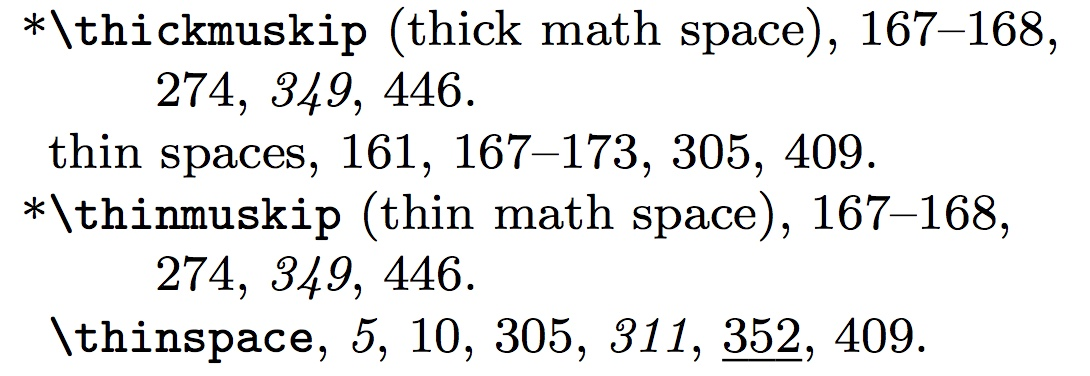
\includegraphics[height=2.5cm]{index.jpg}
    \item \verb+\show+ 명령어로 확인
    \end{itemize}
  \end{itemize}
\end{frame}


%
\begin{frame}[fragile]{매크로 전개}
  다음의 명령어들은 전개 과정에서 전개된다.
  \begin{itemize}
  \item \alert{매크로}
  \item 조건문 (\verb+\if+, \verb+\ifx+, \verb+\ifnum+, \verb+\ifcat+, $\ldots$)
  \item \verb+\number, \romannumeral+
  \item \verb+\string+, \verb+\fontname+, \verb+\jobname+,
    \verb+\meaning+, \verb+\the+
  \item \verb+\csname ... \endcsname+
  \item \verb+\expandafter, \noexpand+
  \item \verb+\topmark+, \verb+\botmark+, \verb+\firstmark+,
    \verb+\splitfirstmark+, \verb+\splitbotmark+
  \item \verb+\input+,  \verb+\endinput+
  \end{itemize}
\end{frame}


%
\begin{frame}[fragile]{매크로 전개}
  매크로가 전개되지 않는 경우
  \begin{itemize}
  \item 매크로 정의 시점, \verb+\def+, \verb+\gdef+, \verb+\edef+, \verb+\xdef+
\begin{Verbatim}[fontsize=\small, formatcom=\color{blue}]
\def\sayhello{Hello, world}
\end{Verbatim}
  \item let 할당문, \verb+\let+ 또는 \verb+\futurelet+,
  {\color{blue} \verb+\let\a=\b+}
  \item 파라미터 텍스트 또는 매크로 인자를 읽어 들일 때
\begin{Verbatim}[fontsize=\small, formatcom=\color{blue}]
\def\foo#1\bar{...}
\foo abc \abc xyz \xyz \bar
\end{Verbatim}
  \item \verb+\def+, \verb+\gdef+로 정의된 치환 텍스트을 읽어 들일 때
\begin{Verbatim}[fontsize=\small, formatcom=\color{blue}] 
\def\hello{Hello, \world}
\edef\hello{Hello, \world} % Error
\end{Verbatim}
  \item \verb+\uppercase+, \verb+\lowercase+ 를 읽어 들일 때
\begin{Verbatim}[fontsize=\small, formatcom=\color{blue}]
\def\say{hello}
\uppercase{\say, abc} => hello, ABC
\uppercase\expandafter{\say, abc} => HELLO, ABC  
\end{Verbatim}
  \end{itemize}
\end{frame}


%
\begin{frame}[fragile]{토큰 리스트}
  \begin{Verbatim*}
\def\tokentwo{\iftrue this \else that \fi}
\def\tokenone#1{...}
...
\expandafter\tokenone\tokentwo
  \end{Verbatim*}
  \bigskip

  \alert{입력 과정}
  
  \fbox{expandafter}\quad
  \fbox{tokenone}\quad
  \fbox{tokentwo}
  
  \bigskip
  \alert{전개 과정}
  
  \fbox{tokenone}\quad
  \verb|t|$_{11}$\quad
  \verb|h|$_{11}$\quad
  \verb|i|$_{11}$\quad
  \verb|s|$_{11}$\quad
  \verb*| |$_{10}$\quad {\color{red} (X)}
  
  \bigskip
  \fbox{tokenone}\quad
  \fbox{iftrue}\quad
  \verb|t|$_{11}$\quad
  \verb|h|$_{11}$\quad
  \verb|i|$_{11}$\quad
  \verb|s|$_{11}$\quad
  \verb*| |$_{10}$\quad
  \fbox{else}\quad
  \verb|t|$_{11}$\quad
  \verb|h|$_{11}$\quad
  \verb|a|$_{11}$\quad
  \verb|t|$_{11}$\quad
  \verb*| |$_{10}$\quad
  \fbox{fi}
\end{frame}


%
\begin{frame}[fragile]{그룹 만들기}
  \textbf{\alert{그룹}}
  \begin{itemize}
  \item \verb+{+, \verb+}+
  \item \verb+\bgroup+, \verb+\egroup+
    {\color{blue}\small \verb+\let\bgroup={ \let\egroup=}+}
  \item \verb+\begingroup+, \verb+\endgroup+ (원시명령어)
    \medskip
    \begin{Verbatim}[fontsize=\small]
  {\bf Hello}
  \bgroup \bf Hello}
  \bf Hello \egroup
  \begingroup \bf Hello} (X)
    \end{Verbatim}
  \end{itemize}
  \begin{Verbatim}[fontsize=\small, formatcom=\color{blue}]
    \def\hello{Hello}
    { \baselineskip=14pt \def\hello{Hola} \hello }
    \hello
    Hola Hello
  \end{Verbatim}
\end{frame}


%
\begin{frame}[standout]
  예제: \texttt{\string\bold} 매크로
\end{frame}


%
\begin{frame}[fragile]{\texttt{\string\bold} 매크로}
  \begin{Verbatim}[formatcom=\color{blue}]
{\bf Hello world}
    
\bold{Hello world}
  \end{Verbatim}
  \begin{alertblock}{Programmer}
    \verb+\def\bold#1{{\bf #1}}+
  \end{alertblock}
\end{frame}


%
\begin{frame}[fragile]{\texttt{\string\bold} 매크로}
  \begin{Verbatim}[fontsize=\small, formatcom=\color{blue}]
\bold{
  Hello

  world
}

Runaway argument?
{ Hello
! Paragraph ended before \bold was complete.
  \end{Verbatim}
  \begin{alertblock}{Programmer first class}
    \verb+\long\def\bold#1{{\bf #1}}+
  \end{alertblock}
\end{frame}


%
\begin{frame}[fragile]{\texttt{\string\bold} 매크로}
  \begin{alertblock}{Hacker}
    \verb+\def\beginbold{\bgroup\bf}+
    
    \verb+\def\endbold{\egroup}+
  \end{alertblock}

  \begin{Verbatim}[fontsize=\small, formatcom=\color{blue}]
\beginbold
Hello

world
\endbold
  \end{Verbatim}
\end{frame}


%
\begin{frame}[fragile]{\texttt{\string\bold} 매크로}
  \begin{alertblock}{Wizard}
    \verb+\def\bold{\bgroup\bf\let\next=}+
  \end{alertblock}

  \begin{Verbatim}[fontsize=\small, formatcom=\color{blue}]
\bold{text}
\bgroup\bf\let\next={text}
  \end{Verbatim}

  \bigskip

  \fbox{bgroup}\quad\fbox{bf}\quad
  \verb|t|$_{11}$\quad\verb|e|$_{11}$\quad
  \verb|x|$_{11}$\quad\verb|t|$_{11}$\quad
  \verb|}|$_{2}$

  \verb|{|$_1$\quad\fbox{bf}\quad
  \verb|t|$_{11}$\quad\verb|e|$_{11}$\quad
  \verb|x|$_{11}$\quad\verb|t|$_{11}$\quad
  \verb|}|$_{2}$
\end{frame}


%
\begin{frame}[standout]
  예제: 스크립트 매크로
\end{frame}


%
\begin{frame}[fragile]{스크립트 매크로}
  \begin{Verbatim}[fontsize=\small]
\beginscript
Now, at last, you can easily typeset
conversations you eavesdrop on in
restaurants and on planes.
  
Really? That's just what I've been waiting
for! How do I do it?
  
Exactly the way this script was done.
  
Is it easy?
  
Extremely.
\endscript
  \end{Verbatim}
\end{frame}


%
\newcount\spk
\def\beginscript{\bgroup \parindent=0pt \color{red} \spk=1 \rightskip.4in
  \def\par{\ifnum\spk=1 \endgraf \color{blue} \spk=2 \leftskip.4in
    \rightskip0in
    \else \endgraf \color{red} \spk=1 \leftskip0in \rightskip.4in \fi}}
\def\endscript {\egroup}

\begin{frame}[fragile]{스크립트 매크로}
  \hsize 3in
  \beginscript
  Now, at last, you can easily typeset
  conversations you eavesdrop on in
  restaurants and on planes.
  
  Really? That's just what I've been waiting
  for! How do I do it?
  
  Exactly the way this script was done.
  
  Is it easy?
  
  Extremely.
  \endscript
\end{frame}


%
\begin{frame}[fragile]{스크립트 매크로}
  \begin{Verbatim}[fontsize=\small]
\let\endgraf=\par
\newcount\spk
\def\beginscript{\bgroup \parindent=0pt \color{red}
  \spk=1 \rightskip.4in
  \def\par{\ifnum\spk=1 \endgraf \color{blue} \spk=2
             \leftskip.4in \rightskip0in
           \else \endgraf \color{red} \spk=1
             \leftskip0in \rightskip.4in \fi}}
\def\endscript{\egroup}
  \end{Verbatim}
\end{frame}


%
\begin{frame}{참고 문서}
  \begin{itemize}
  \item \href{http://ftp.ktug.org/tex-archive/systems/knuth/dist/tex/}
    {The \TeX book}
  \item \href{https://www.tug.org/TUGboat/tb08-3/tb19knut.pdf}
    {Macros for Jill}
  \end{itemize}
\end{frame}


%
\begin{frame}[standout]
  Any questions?
\end{frame}

\end{document}
